% 05_reti_neurali.tex — Capitolo 5: Reti neurali: dal neurone al MLP.
% Documento didattico "Intelligenza artificiale nel progetto supervised_telemedicina".

\chapter{Reti neurali: dal neurone al MLP}\label{cap:reti}

Nei capitoli precedenti abbiamo visto come il teacher rule-based assegni una
classe di rischio (\classe{basso}, \classe{medio}, \classe{alto}) a partire
da sei parametri vitali e come il progetto \progetto{} abbia generato un
dataset sintetico etichettato da quelle regole (capitolo~\ref{cap:teacher}).
In questo capitolo entriamo nel cuore del progetto: la rete neurale che deve
\textit{imitare} il teacher. Partiamo dal singolo neurone artificiale e
costruiamo, passo dopo passo, il percettrone multistrato (MLP) implementato
in \file{src/telemedicina\_supervised/ml/mlp.py}.

\section{Il neurone artificiale}\label{sec:neurone-artificiale}

Un neurone artificiale è una funzione che riceve un vettore di input
$x = (x_1, \dots, x_d)$, lo combina linearmente con un vettore di pesi $w$ e
un bias $b$, e infine applica una funzione di attivazione non lineare
$\sigma$:

\begin{equation}
z = w \cdot x + b = \sum_{i=1}^{d} w_i x_i + b, \qquad
a = \sigma(z).
\end{equation}

Per chi programma, è utile pensare al neurone come a una funzione composta:
prima una \emph{combinazione lineare} (un prodotto scalare più una costante),
poi una \emph{non linearità} applicata al risultato. Senza la seconda parte
il neurone sarebbe solo una retta (o un iperpiano) nello spazio delle
feature: utile, ma incapace di rappresentare relazioni più ricche.

Nel progetto \progetto{} ogni campione è un vettore di sei feature (la
pressione sistolica, la diastolica, la frequenza cardiaca, la temperatura,
la saturazione di ossigeno e la glicemia), nell'ordine definito dal contratto
in \file{src/telemedicina\_supervised/safety/safety\_rules.py}. Prima di
entrare nella rete, le feature vengono \emph{standardizzate} dallo scaler
(\file{src/telemedicina\_supervised/ml/scaler.py}): ogni colonna viene
trasformata in $(x - \mu)/\sigma$, dove $\mu$ e $\sigma$ sono media e
deviazione standard calcolate \emph{solo} sul train. La rete lavora quindi
su valori con media zero e varianza unitaria, come vedremo nel
capitolo~\ref{cap:training}.

La funzione di attivazione usata dallo strato nascosto del nostro MLP è la
ReLU (Rectified Linear Unit):

\begin{equation}
\mathrm{ReLU}(z) = \max(0, z).
\end{equation}

La ReLU è la più semplice delle non linearità: azzera i valori negativi e
lascia passare quelli positivi. È l'equivalente di un
\codice{if z > 0: a = z else: a = 0} in Python, ma scritto in forma
vettoriale.

\section{Perché serve la non linearità}\label{sec:non-linearita}

Una domanda naturale è: perché complicarsi la vita con una non linearità?
La risposta è matematica e ha un'analogia diretta con la programmazione.
Una composizione di trasformazioni lineari è ancora una trasformazione
lineare: se $f(x) = W_1 x + b_1$ e $g(y) = W_2 y + b_2$, allora
$g(f(x)) = (W_2 W_1) x + (W_2 b_1 + b_2)$, cioè una sola trasformazione
lineare con matrice $W_2 W_1$ e bias $W_2 b_1 + b_2$.

In termini di codice: concatenare due funzioni che fanno solo
\codice{return W @ x + b} produce una funzione che fa ancora
\codice{return W2 @ (W1 @ x + b1) + b2}, ovvero
\codice{return (W2 @ W1) @ x + ...}. Non importa quanti strati lineari si
impilano: il risultato è sempre un singolo strato lineare. Per rappresentare
relazioni non lineari (come le soglie del teacher, che sono \emph{confini
netti} nello spazio delle feature) serve almeno una non linearità tra uno
strato e l'altro.

La ReLU, in particolare, introduce dei ``ginocchi'' nella funzione appresa:
la rete può ``piegare'' lo spazio delle feature in corrispondenza dei punti
in cui $z$ cambia segno. Con più neuroni e più strati, queste piegature si
combinano e la rete può approssimare confini di decisione arbitrariamente
complessi (capitolo~\ref{cap:distillazione}).

\section{Dal neurone alla rete}\label{sec:dal-neurone-alla-rete}

Un MLP è una composizione di strati di neuroni. Il nostro modello ha due
strati:

\begin{itemize}
  \item uno \emph{strato nascosto} di $n$ neuroni ReLU, che riceve le 6
        feature standardizzate;
  \item uno \emph{strato di output} di 3 neuroni softmax, uno per classe
        (\classe{basso}, \classe{medio}, \classe{alto}).
\end{itemize}

L'architettura si scrive in breve come $6 \to n \to 3$. Il codice reale del
forward pass, in \file{src/telemedicina\_supervised/ml/mlp.py}, è il
seguente:

\begin{lstlisting}[caption={Forward pass del MLP in \file{mlp.py} (metodo \codice{forward}).}]
def forward(self, X: np.ndarray) -> Dict[str, np.ndarray]:
    z1 = X @ self.W1.T + self.b1
    a1 = np.maximum(z1, 0.0)  # ReLU
    z2 = a1 @ self.W2.T + self.b2
    # Softmax stabile: sottrae il massimo per riga.
    z2_shiftati = z2 - np.max(z2, axis=1, keepdims=True)
    esponenziali = np.exp(z2_shiftati)
    probs = esponenziali / np.sum(esponenziali, axis=1, keepdims=True)
    return {"z1": z1, "a1": a1, "z2": z2, "probs": probs}
\end{lstlisting}

Le righe del codice corrispondono esattamente alla teoria:

\begin{itemize}
  \item \codice{z1 = X @ self.W1.T + self.b1}: la somma pesata
        $z_1 = W_1 x + b_1$ per tutti i campioni in un colpo solo (le
        matrici in numpy vettorizzano il calcolo);
  \item \codice{a1 = np.maximum(z1, 0.0)}: la ReLU applicata elemento per
        elemento;
  \item \codice{z2 = a1 @ self.W2.T + self.b2}: la somma pesata del secondo
        strato, che produce i \emph{logit} grezzi;
  \item le ultime righe: la softmax, che trasforma i logit in probabilità.
\end{itemize}

\begin{esempio}{Il forward pass in \progetto{}}
Il metodo \codice{forward} riceve una matrice \codice{X} di forma
\codice{(n\_campioni, 6)} e restituisce un dizionario con le attivazioni
intermedie (\codice{z1}, \codice{a1}, \codice{z2}) e le probabilità finali
(\codice{probs}). I metodi \codice{probabilità}, \codice{predici\_indici} e
\codice{predici\_etichette} sono semplici wrapper attorno a \codice{forward}:
rispettivamente restituiscono le probabilità softmax, l'indice della classe
più probabile (\codice{np.argmax}) e la relativa etichetta stringa.
\end{esempio}

\section{La softmax come probabilità}\label{sec:softmax}

L'ultimo strato non applica una ReLU ma una \emph{softmax}. Dato un vettore
di logit $z = (z_1, z_2, z_3)$, la softmax produce:

\begin{equation}
p_i = \frac{e^{z_i}}{\sum_{j=1}^{3} e^{z_j}}, \qquad i = 1, 2, 3.
\end{equation}

Due proprietà rendono la softmax ideale per la classificazione:

\begin{itemize}
  \item l'esponenziale rende ogni $e^{z_i}$ positivo, quindi le probabilità
        sono tutte $> 0$;
  \item la normalizzazione per la somma fa sì che $\sum_i p_i = 1$: le tre
        uscite formano una distribuzione di probabilità.
\end{itemize}

Si può leggere $p_i$ come la \emph{fiducia} del modello nella classe $i$:
se $p = (0.02, 0.03, 0.95)$ il modello è molto sicuro che il campione sia
\classe{alto}; se $p = (0.34, 0.33, 0.33)$ è incerto. Questa lettura
probabilistica non è solo elegante: nel capitolo~\ref{cap:sicurezza}
vedremo che il progetto usa proprio la confidenza softmax (la probabilità
massima) per decidere quando fidarsi dell'MLP e quando ripiegare sulle
regole del safety gate.

Nel codice, la softmax è resa \emph{numericamente stabile} sottraendo il
massimo dei logit prima dell'esponenziale:
\codice{z2\_shiftati = z2 - np.max(z2, axis=1, keepdims=True)}. Senza
questa accortezza, logit grandi potrebbero far esplodere \codice{np.exp} in
overflow.

\section{Il MLP del progetto in pratica}\label{sec:mlp-progetto}

La figura~\ref{fig:architettura} mostra l'architettura completa, e il
diagramma TikZ in figura~\ref{fig:architettura-tikz} la riassume con i nomi
delle matrici dei pesi.

\begin{figure}[htbp]
  \centering
  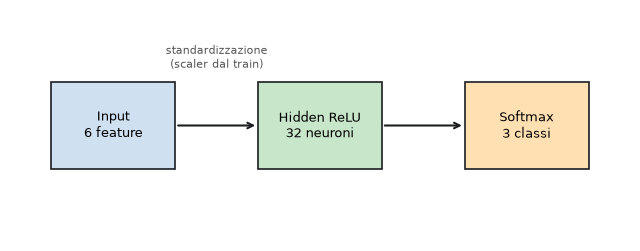
\includegraphics[width=0.85\textwidth]{figure/generate/architettura.png}
  \caption{Architettura del MLP di \progetto{}: 6 feature in ingresso, uno
  strato nascosto ReLU con $n$ neuroni e uno strato di output softmax con 3
  classi.}
  \label{fig:architettura}
\end{figure}

\begin{figure}[htbp]
  \centering
  % diagramma_architettura.tex — diagramma TikZ (incluso dai capitoli).
\begin{tikzpicture}[
    nodo/.style={draw, rounded corners=2pt, minimum height=0.9cm, align=center, font=\small},
    freccia/.style={-{Stealth[length=2.5mm]}, thick},
  ]
  \node[nodo, fill=blue!10] (in) at (0,0) {Input\\6 feature};
  \node[nodo, fill=green!15] (hid) at (4,0) {Hidden ReLU\\$n$ neuroni};
  \node[nodo, fill=orange!15] (out) at (8,0) {Softmax\\3 classi};
  \draw[freccia] (in) -- (hid) node[midway, above, font=\scriptsize] {$W_1, b_1$};
  \draw[freccia] (hid) -- (out) node[midway, above, font=\scriptsize] {$W_2, b_2$};
  \node[below=0.35cm of in, font=\scriptsize, align=center] {standardizzazione\\con lo scaler};
\end{tikzpicture}

  \caption{Schema del MLP con le matrici dei pesi: $W_1$ (da 6 a $n$),
  $W_2$ (da $n$ a 3) e i rispettivi bias.}
  \label{fig:architettura-tikz}
\end{figure}

Quanti parametri ha il modello? Contiamo pesi e bias:

\begin{itemize}
  \item $W_1$: $n \times 6$ pesi (dallo strato di input a quello nascosto);
  \item $b_1$: $n$ bias;
  \item $W_2$: $3 \times n$ pesi (dallo strato nascosto a quello di output);
  \item $b_2$: $3$ bias.
\end{itemize}

In totale: $6n + n + 3n + 3 = 10n + 3$ parametri. Con la configurazione
migliore del progetto ($n = 32$, vedi capitolo~\ref{cap:training}) si hanno
$10 \cdot 32 + 3 = 323$ parametri: un modello molto piccolo, addestrabile
in pochi secondi su una CPU.

\begin{esempio}{Quanti parametri ha il modello?}
Con $n = 32$: $W_1$ ha $32 \times 6 = 192$ pesi, $b_1$ ha 32 elementi,
$W_2$ ha $3 \times 32 = 96$ pesi e $b_2$ ha 3 elementi. Somma:
$192 + 32 + 96 + 3 = 323$. Il modello è volutamente piccolo: deve
approssimare un teacher deterministico, non scoprire pattern complessi da
dati reali \cite{progetto2026}.
\end{esempio}

\section{Perché una rete può imparare relazioni non lineari}\label{sec:relazioni-non-lineari}

Il teacher rule-based del capitolo~\ref{cap:teacher} classifica con
\emph{soglie nette}: per esempio, la glicemia $\geq 200$ contribuisce a una
classe \classe{alto}, altrimenti no. Il confine tra le classi è un
iperpiano perpendicolare all'asse della feature: una regola del tipo
\codice{if glicemia >= 200: alto}.

Un MLP con ReLU non è limitato a confini rettilinei. Ogni neurone nascosto
definisce un ``ginocchio'' nello spazio delle feature; combinando più
neuroni, la rete può tracciare confini di decisione \emph{curvi} e
approssimare la funzione del teacher anche dove le soglie si combinano in
modo complesso (per esempio quando più parametri sono simultaneamente fuori
range). Questa capacità di approssimare funzioni non lineari è il motivo per
cui l'MLP può \emph{imitare} il teacher: nel capitolo~\ref{cap:distillazione}
vedremo come il progetto sfrutti questa proprietà per distillare la
conoscenza delle regole in una rete addestrata su dati etichettati dal
teacher stesso. Come scrivono Goodfellow e colleghi, le reti profonde
costruiscono rappresentazioni gerarchiche in cui ogni strato trasforma
l'input in una forma più adatta al compito \cite{goodfellow2016deep}.